\begin{center}
	\begin{tabular}{M{9.25cm}M{8.75cm}}
		\textbf{TRƯỜNG THCS-THPT NGUYỄN KHUYẾN}& \textbf{ÔN TẬP KIỂM TRA GIỮA HỌC KÌ II}\\
		\textbf{MÃ ĐỀ: 002}& \textbf{Bài thi môn: VẬT LÝ 10}\\
		\textit{(Đề thi có 03 trang)}& \textit{Thời gian làm bài: 45 phút, không kể phát đề}
		
		\noindent\rule{4cm}{0.8pt} \\
	\end{tabular}
\end{center}
\setcounter{section}{0}
\section{Câu trắc nghiệm nhiều phương án lựa chọn}
\textit{Thí sinh trả lời từ câu 1 đến câu 12. Mỗi câu hỏi thí sinh chọn một phương án}
\setcounter{ex}{0}
\Opensolutionfile{ans}[ans/D10-GK-HK2-002-TN]
% ===================================================================
\begin{ex}
	Phát biểu nào sau đây là \textbf{sai} khi nói về năng lượng?
	\choice
	{Năng lượng là một đại lượng vô hướng}
	{Năng lượng có thể chuyển hoá từ dạng này sang dạng khác}
	{Năng lượng luôn là một đại lượng bảo toàn}
	{\True Trong hệ SI, đơn vị của năng lượng là cal}
	\loigiai{}
\end{ex}
% ===================================================================
\begin{ex}
	Công là đại lượng
	\choice
	{\True vô hướng, có thể âm, dương hoặc bằng không}
	{vô hướng, có thể âm hoặc dương}
	{vector, có thể âm, dương hoặc bằng không}
	{vector, có thể âm hoặc dương}
	\loigiai{}
\end{ex}
% ===================================================================
\begin{ex}
	Cơ năng của vật sẽ \textbf{không được} bảo toàn khi vật
	\choice
	{chỉ chịu tác dụng của trọng lực}
	{chỉ chịu tác dụng của lực đàn hồi của lò xo}
	{\True chịu tác dụng của lực cản, lực ma sát}
	{không chịu tác dụng của lực ma sát, lực cản và các loại lực không phải lực thế}
	\loigiai{}
\end{ex}`
% ===================================================================
\begin{ex}
	Một lực $\vec{F}$ không đổi liên tục kéo một vật chuyển động với vận tốc $\vec{v}$ theo hướng của lực. Công suất của lực $\vec{F}$ là
	\choice
	{\True $Fv$}
	{$Fv^2$}
	{$Fvt$}
	{$Ft$}
	\loigiai{}
\end{ex}

% ===================================================================
\begin{ex}
	Thế năng trọng trường của một vật có giá trị
	\choice
	{luôn dương}
	{luôn âm}
	{khác 0}
	{\True có thể dương, có thể âm hoặc bằng 0}
	\loigiai{}
\end{ex}
% ===================================================================
\begin{ex}
	Một vật chịu tác dụng của một lực $F$ không đổi có độ lớn \SI{5}{\newton}, phương của lực hợp với phương chuyển động một góc \SI{60}{\degree}. Biết rằng quãng đường đi được là \SI{6}{\meter}. Công của lực $F$ là
	\choice
	{\SI{11}{\joule}}
	{\SI{50}{\joule}}
	{\SI{30}{\joule}}
	{\True \SI{15}{\joule}}
	\loigiai{
		$A=F\cdot S \cdot cos \alpha = \SI{15}{\joule} $
	}
\end{ex}


% ===================================================================
\begin{ex}
	Có ba chiếc xe ô tô với khối lượng và vận tốc lần lượt là:
	\begin{center}
		\renewcommand{\arraystretch}{1.8}
		\begin{tabular}{|M{5cm}|M{5cm}|M{5cm}|}
			\hline
			Xe A: $m$, $v$;&Xe B: $\dfrac{m}{2}$, $3v$; &Xe C: $3m$, $\dfrac{v}{2}$.\\
			\hline
		\end{tabular}
	\end{center}
	Thứ tự các xe theo thứ tự động năng tăng dần là
	\choice
	{A, B, C}
	{B, C, A}
	{\True  C, A, B}
	{C, B, A}
	\loigiai{}
\end{ex}
% ===================================================================
\begin{ex}
	Từ mặt đất người ta ném một vật lên cao với tốc độ $\SI{10}{\meter/\second}$. Nếu bỏ qua mọi ma sát và lấy $g=\SI{10}{\meter/\second^2}$ thì độ cao lớn nhất mà vật có thể lên tới là
	\choice
	{\True \SI{5}{\meter}}
	{\SI{10}{\meter}}
	{\SI{0.5}{\meter}}
	{\SI{50}{\meter}}
	\loigiai{}
\end{ex}
% ===================================================================
\begin{ex}
	Một vận động viên nhảy cầu nhảy xuống hồ nước từ tấm ván ở độ cao \SI{10}{\meter} so với mặt hồ. Lấy $g=\SI{9.8}{\meter/\second^2}$. Tốc độ của người khi cách mặt hồ \SI{4}{\meter} là
	\choice
	{\SI{14.14}{\meter/\second}}
	{\SI{8.94}{\meter/\second}}
	{\True \SI{10.84}{\meter/\second}}
	{\SI{7.7}{\meter/\second}}
	\loigiai{}
\end{ex}
% ===================================================================
\begin{ex}
	Một chiếc xe mô tô có khối lượng \SI{220}{\kilogram} đang chạy với tốc độ \SI{14}{\meter/\second}. Công cần thực hiện để tăng tốc xe lên tốc độ \SI{19}{\meter/\second} là bao nhiêu?
	\choice
	{\True \SI{18150}{\joule}}
	{\SI{21560}{\joule}}
	{\SI{39710}{\joule}}
	{\SI{2750}{\joule}}
	\loigiai{}
\end{ex}
% ===================================================================
\begin{ex}
	Khi một ô tô di chuyển với vận tốc không đổi trên đường cao tốc, phần lớn công suất do động cơ tạo ra được sử dụng để bù đắp cho sự mất mát năng lượng cơ học do các lực cản tác dụng lên xe từ không khí và mặt đường. Nếu công suất do động cơ tạo ra là \SI{175}{HP}, hãy ước tính tổng lực ma sát tác dụng lên xe khi nó đang di chuyển với tốc độ $\SI{29}{\meter / \second}$.
	\choice
	{\True $\SI{4502}{\newton}$}
	{$\SI{3806}{\newton}$}
	{$\SI{2401}{\newton}$}
	{$\SI{6605}{\newton}$}
	\loigiai{
		
	}
\end{ex}
% ===================================================================
\begin{ex}
	\immini{Thùng hàng có khối lượng $\SI{3}{\kilogram}$ trượt xuống một mặt phẳng nghiêng. Mặt phẳng nghiêng có chiều dài $\SI{1}{\meter}$ và nghiêng một góc $\SI{30}{\degree}$ như hình bên. Thùng hàng bắt đầu từ trạng thái nghỉ ở đỉnh, chịu tác dụng của một lực ma sát không đổi có độ lớn $\SI{5}{\newton}$. Lấy gia tốc trọng trường $g=\SI{9.8}{\meter/\second^2}$. Tốc độ của thùng hàng tại chân mặt phẳng nghiêng là 
		\choice
		{\True $\SI{2.54}{\meter / \second}$}
		{$\SI{3.65}{\meter / \second}$}
		{$\SI{4.23}{\meter / \second}$}
		{$\SI{1.61}{\meter / \second}$}}
	{\vspace{-0.5cm}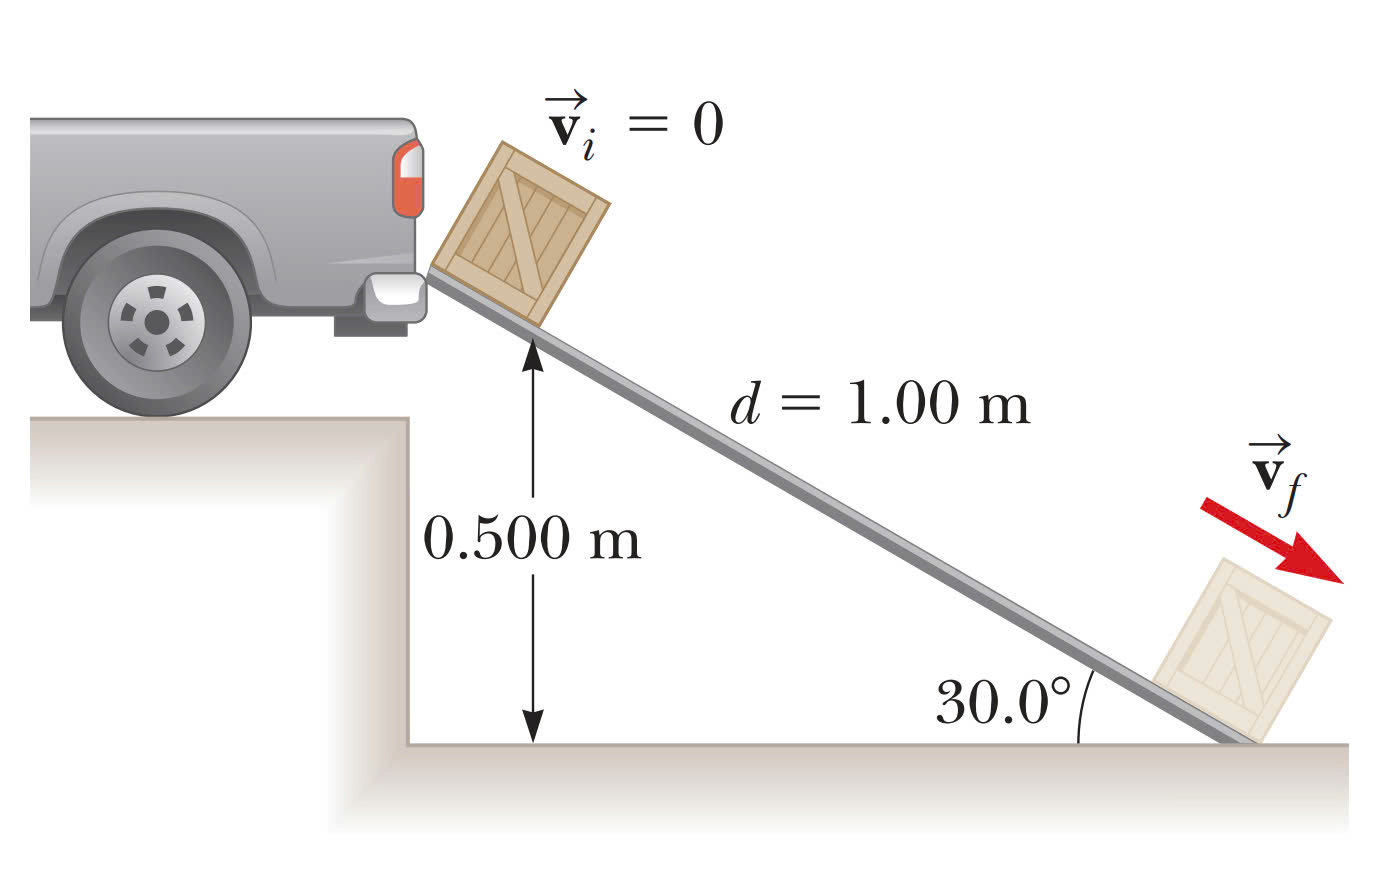
\includegraphics[scale=0.1]{../figs/LTTHPT-TOPIC3-13}}
	\loigiai{
		
	}
\end{ex}
\Closesolutionfile{ans}
\section{Câu trắc nghiệm đúng/sai} 
\textit{Thí sinh trả lời từ câu 1 đến câu 4. Trong mỗi ý \textbf{a)}, \textbf{b)}, \textbf{c)}, \textbf{d)} ở mỗi câu, thí sinh chọn đúng hoặc sai}
\setcounter{ex}{0}\\
\Opensolutionfile{ans}[ans/D10-GK-HK2-002-TF]
% ===================================================================
\begin{ex}
	Người ta đẩy một cái thùng gỗ có khối lượng $\SI{55}{\kilogram}$ theo phương ngang với lực không đổi có độ lớn $\SI{220}{\newton}$ làm thùng bắt đầu chuyển động trên mặt phẳng ngang cùng hướng với lực tác dụng. Hệ số ma sát trượt giữa thùng và mặt phẳng là $\SI{0.35}{}$. Lấy $g =\SI{10}{\meter/\second^2}$.
	\choiceTF
	{Thùng trượt đều trên sàn}
	{\True Công của lực đẩy khi thùng di chuyển được $\SI{1}{\meter}$ là $\SI{220}{\joule}$}
	{\True Công của lực ma sát trượt khi thùng di chuyển được $\SI{2}{\meter}$ là $\SI{-385}{\joule}$
	}
	{Sau khi di chuyển được $\SI{2}{\meter}$ kể từ thời điểm bắt đầu trượt, tốc độ của thùng là $\SI{2}{\meter/\second}$}
	\loigiai{
		\begin{itemchoice}
			\itemch Sai. Thùng trượt với gia tốc $a=\dfrac{F-\mu mg}{m}=\SI{0.5}{\meter/\second^2}$.
			\itemch Đúng.
			\itemch Đúng.
			\itemch Sai. $A_{F}-A_{F_{\mathrm{ms}}}=\dfrac{1}{2}mv^2\Rightarrow v=\xsi{\sqrt{2}}{\meter/\second}$.
		\end{itemchoice}
	}
\end{ex}
% ===================================================================
\begin{ex}
	\immini{Một viên bi nhỏ được coi là chất điểm có khối lượng $\SI{5}{\kilogram}$ được thả từ trạng thái nghỉ tại điểm A và trượt trên một đoạn đường không có ma sát như hình bên. Lấy gia tốc trọng trường $g=\SI{9.8}{\meter/\second^2}$.
		\choiceTF
		{Không thể áp dụng định luật bảo toàn cơ năng cho trường hợp này}
		{\True Tốc độ tại điểm B là $\SI{5.94}{\meter / \second}$}
		{\True Tốc độ tại điểm C là $\SI{7.67}{\meter / \second}$}
		{Công của trọng lực khi vật đi từ A đến C là $W_P=\SI{280}{\joule}$}}{\vspace{-0.5cm}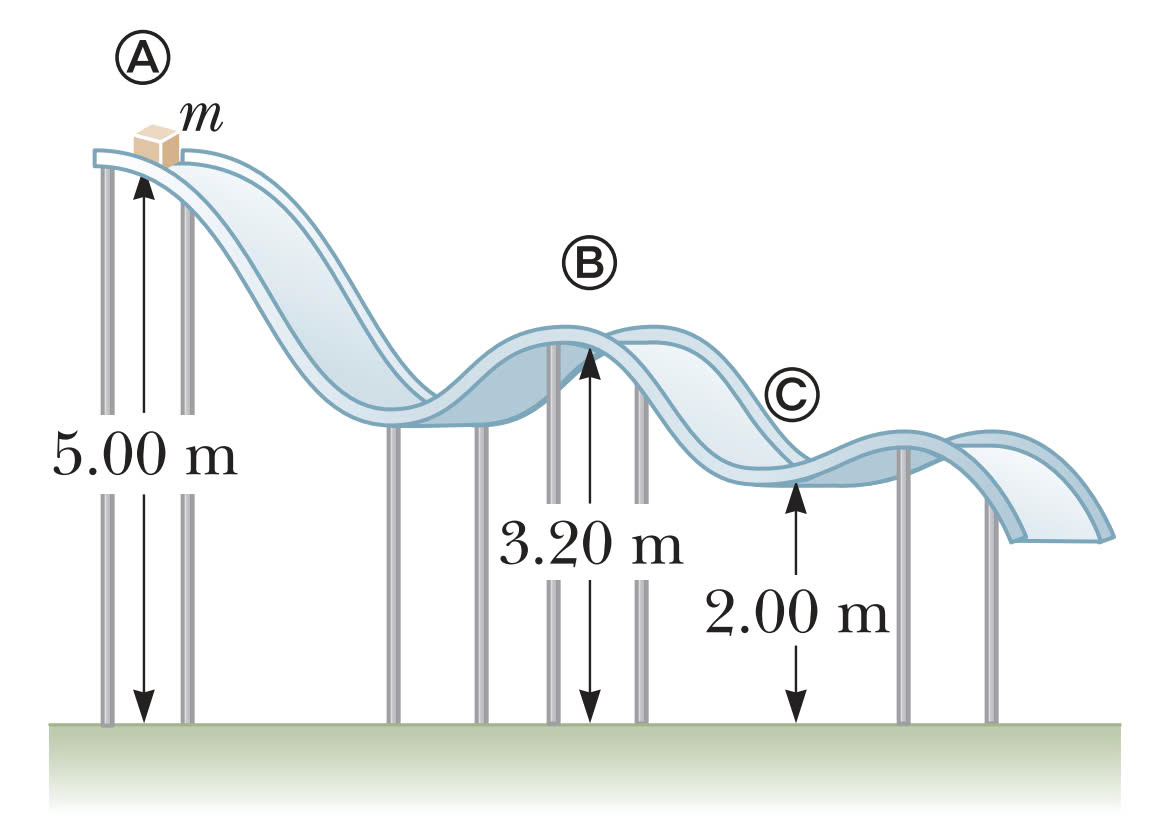
\includegraphics[scale=0.1]{../figs/LTTHPT-TOPIC3-8}}
	\loigiai{
		\begin{enumerate}[label=\alph*)] %alph=> arabic nếu muốn sử dụng số
			\item Sai. Vật chỉ chịu tác dụng của trọng lực => Có thể áp dụng định luật bảo toàn cơ năng
			\item Đúng. $v_B=\sqrt{2g(h_A-h_B)}=\SI{5.94}{\meter / \second}$
			\item Đúng. $v_C=\sqrt{2g(h_A-h_C)}=\SI{7.67}{\meter / \second}$
			\item Sai. $W_P=mg(h_A-h_C)=\SI{147}{\joule}$
		\end{enumerate}
	}
\end{ex}
% ===================================================================
\begin{ex}
	Tại một nơi có gia tốc trọng trường $g=\SI{10}{\meter/\second^2}$, thả một vật có khối lượng $\SI{5}{\kilogram}$ tại vị trí có thế năng trọng trường bằng $W_{\text{t1}}=\SI{600}{\joule}$, khi đến mặt đất thì thế năng của vật bằng $W_{\text{t2}}=\SI{-1000}{\joule}$. Bỏ qua mọi ma sát.
	\choiceTF
	{Sau khi thả vật thì động năng tăng dần, cơ năng giảm dần}
	{\True Vật đã rơi từ độ cao $\SI{32}{\meter}$ so với mặt đất} 
	{Gốc thế năng đã chọn ở độ cao $\SI{10}{\meter}$ so với mặt đất}
	{Tốc độ của vật tại gốc thế năng là $\xsi{2\sqrt{15}}{\meter/\second}$}
	\loigiai{
		\begin{itemchoice}
			\itemch Sai. Cơ năng của vật không đổi.
			\itemch Đúng. Ta có $W_{\text{t1}}-W_{\text{t2}}=mg\Delta h\Rightarrow \Delta h=\dfrac{W_{\text{t1}}-W_{\text{t2}}}{mg}=\SI{32}{\meter}$.
			\itemch Sai. Tại vị trí gốc thế năng thì $h=0$.\\
			$$h_1=\dfrac{W_{\text{t1}}}{mg}=\SI{12}{\meter}.$$
			Gốc thế năng đã chọn ở độ cao $\SI{20}{\meter}$ so với mặt đất.
			\itemch Sai. Tốc độ của vật tại gốc thế năng: $v=\sqrt{2gh_1}=\xsi{4\sqrt{15}}{\meter/\second}$.
		\end{itemchoice}
	}
\end{ex}
% ===================================================================
\begin{ex}
	\immini{Khi thực hiện tư thế bật nhảy, người ta sẽ trải qua 2 giai đoạn: nhún chân tạo đà và bay trên không. Để khảo sát chuyển động của người nhảy một cách đơn giản, người ta có thể mô tả chuyển động thông qua chuyển động của khối tâm CM (center of mass). Hình bên biểu diễn vị trí và tốc độ khối tâm ở các giai đoạn tương ứng của cú nhảy. Một học sinh nam thực hiện giai đoạn nhún chân tạo đà và tăng tốc đều trên đoạn $h=\SI{0.40}{\meter}$ trong khoảng thời gian $\Delta t=\SI{0.25}{\second}$. Nam sinh có khối lượng \SI{68}{\kilogram}. Lấy gia tốc trọng trường $g=\SI{9.80}{\meter/\second^2}$. }
	{\vspace{-0.5cm}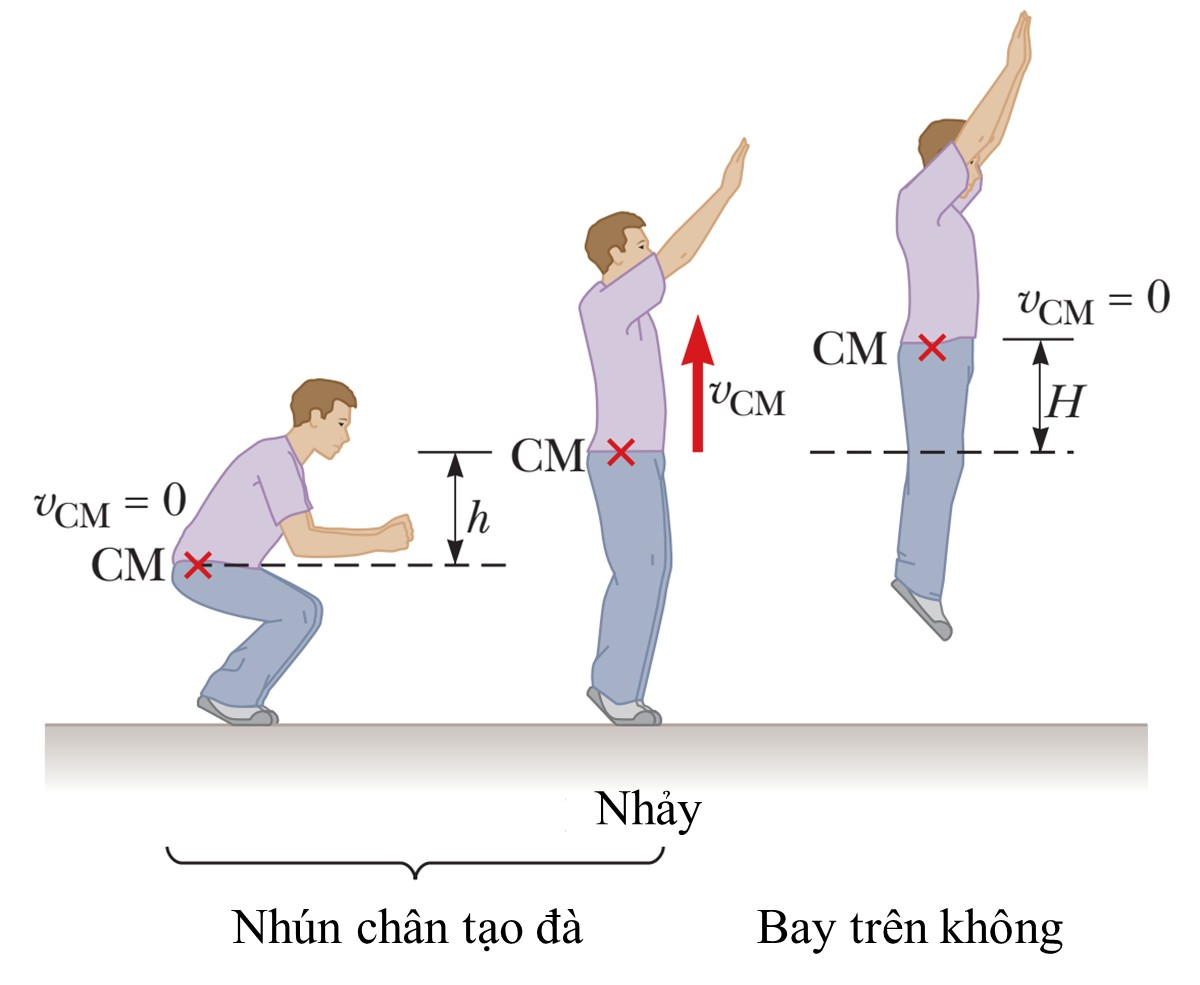
\includegraphics[scale=0.35]{../figs/D10-GK-HK2-4}}
	\choiceTF
	{\True Tốc độ của bạn học sinh khi vừa bật khỏi đất là \SI{3.2}{\meter/\second}}
	{Trong quá trình nhảy lên, cơ năng của bạn học sinh tăng dần}
	{Độ cao cực đại mà bạn học sinh đạt được là $H=\SI{0.13}{\meter}$}
	{\True Biết rằng cơ bắp con người chỉ có hiệu suất tối đa là \SI{25}{\percent} trong việc tạo ra động năng từ năng lượng hóa học (năng lượng cung cấp từ thực phẩm). Để thực hiện được cú nhảy trên thì nam sinh cần được cung cấp ít nhất \SI{83.2}{cal}}
	\loigiai{}
\end{ex}
\Closesolutionfile{ans}
\section{Tự luận} 
\setcounter{ex}{0}
\Opensolutionfile{ans}[ans/D10-GK-HK2-002-TL]
% ===============================================================
\begin{ex}
	Thùng hàng có khối lượng $\SI{70}{\kilogram}$ được kéo lên một dốc bằng một sợi cáp chạy bằng động cơ. Nếu thùng hàng này được kéo lên $\SI{60}{\meter}$ trên một dốc nghiêng $\SI{30}{\degree}$ với tốc độ không đổi $\SI{2}{\meter/\second}$ và bỏ qua mọi ma sát thì công suất của động cơ để thực hiện việc này là bao nhiêu mã lực? Lấy $g=\SI{9.8}{\meter/\second^2}$. \textit{(Kết quả làm tròn đến chữ số hàng phần trăm)}.
	\loigiai{
		$W=mgsin\theta\cdot d=\SI{20538}{\joule}$\\
		$P_{hp}=\dfrac{W}{t.746}=\SI{0.92}{HP}$.
	}
\end{ex}
% ===================================================================
\begin{ex}
	Một vật có khối lượng $\SI{1500}{\gram}$ thả không vận tốc đầu từ đỉnh dốc nghiêng cao $\SI{2}{\meter}$. Lấy $g=\SI{9.8}{\meter / \second\squared}$.
	\begin{enumerate}[label=\alph*)]
		\item Bỏ qua mọi ma sát, tính tốc độ của vật khi đến chân dốc nghiêng.
		\item Do ma sát nên tốc độ vật ở chân dốc chỉ bằng $\dfrac{2}{3}$ tốc độ của vật đến chân dốc khi không có ma sát. Công của lực ma sát là bao nhiêu?
	\end{enumerate}
	\loigiai{
	\begin{enumerate}[label=\alph*)]
		\item $v_c\approx\SI{6.26}{\meter/\second}$.
		\item $A_{F_{\mathrm{ms}}}=\SI{-16.33}{\joule}$.
	\end{enumerate}
	}
\end{ex}
% ===================================================================
\begin{ex}
	Cho một con lắc đơn gồm: sợi dây (khối lượng không đáng kể) dài $\SI{320}{\centi \meter}$, đầu trên cố định, đầu dưới treo một vật nặng có khối lượng $\SI{1000}{\gram}$. Khi vật đang ở vị trí cân bằng thì truyền cho vật một vận tốc là $\xsi{4\sqrt{2}}{\meter/\second}$ theo phương ngang. Lấy $g=\SI{10}{\meter / \second \squared}$, bỏ qua lực cản của không khí. 
	\begin{enumerate}[label=\alph*)]
		\item Tính cơ năng ban đầu của vật nặng.
		\item Xác định tốc độ của vật ở vị trí dây lệch với phương thẳng đứng góc $\SI{30}{\degree}$.
		\item Ở vị trí có góc lệch bao nhiêu so với phương thẳng đứng thì thế năng của vật nặng gấp 2 lần động năng?
	\end{enumerate}
	\textit{(Kết quả làm tròn đến chữ số hàng phần mười).}
	\loigiai{
		\begin{enumerate}[label=\alph*)]
			\item $W=\SI{16}{\joule}$.
			\item $v\approx\SI{4.84}{\meter/\second}$.
			\item $\alpha=\SI{48.2}{\degree}$.
		\end{enumerate}
	}
\end{ex}
\Closesolutionfile{ans}
\begin{center}
	\textbf{--- HẾT ---}
\end{center}